\section{Iterators}

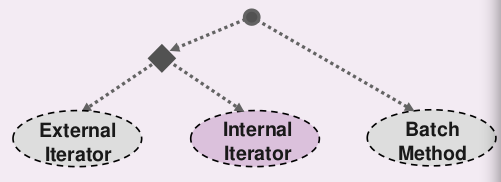
\includegraphics[width=0.7\linewidth]{iterators.png}

\subsection{External Iterator}

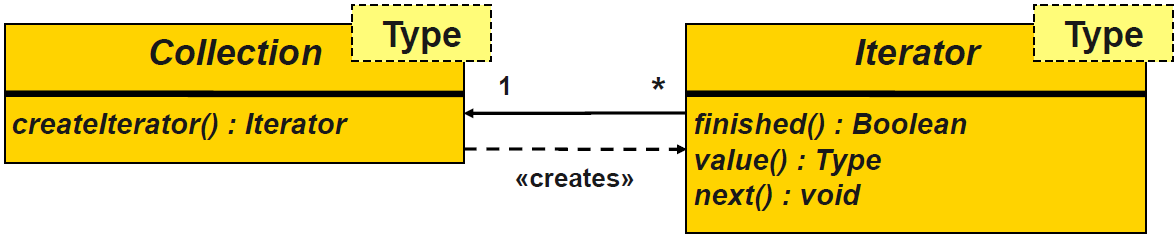
\includegraphics[width=\linewidth]{external_iterator.png}

\subsubsection{Problem}
\begin{itemize}
    \item Iteration through a collection depends on the target implementation
    \item Separate logic of iteration into an object to allow multiple iteration strategies
\end{itemize}

\subsubsection{Intent}
Wie kann eine starke Kopplung zwischen Iteration und Sammlung vermieden, verallgemeinert und auf eine sammlungsoptimierte Weise bereitgestellt werden?

\subsubsection{Solution}
Biete einen Weg um auf Elemente eines aggregierten Objekts sequenziell zuzugreifen, ohne die darunterliegende Repräsentation aufzudecken \\

\textbf{Elementary operations of an Iterator's behaviour}
\begin{itemize}
    \item Initializing an iteration \textit{new ArrayList().iterator();}
    \item Checking a completion condition \textit{it.hasNext();}
    \item Accessing a current target value \textit{var x = it.next();}
    \item Moving to the next target value \textit{it.next();}
\end{itemize}
\vspace{10pt}
\textbf{Known uses}

\begin{itemize}
    \item C++ it.hasNext()
    \item For-Each Statements
\end{itemize}

\subsubsection{Consequences}
\textbf{Benefits}
\begin{itemize}
    \item Bietet eine einzige Schnittstelle um durch jede Art von Collection zu iterieren
\end{itemize}
\vspace{10pt}
\textbf{Liabilities}
\begin{itemize}
    \item Mehrere Iteratoren loopen durch eine Collection zur selben Zeit $\rightarrow$ Robustheit ist schwer zu erreichen, wenn sich die Collection ändert
    \item Life-Cycle Management von Iterator Objekten $\rightarrow$ Braucht vielleicht Disposal-Methode oder Iterator muss die Collection überwachen
    \item Enge Kopplung zwischen Iterator und zugehöriger Collection-Klasse
    \item Indexing kann intuitiver sein für Programmierer
\end{itemize}

\vfill\null
\columnbreak

\subsection{Enumeration Method / Internal Iterator}

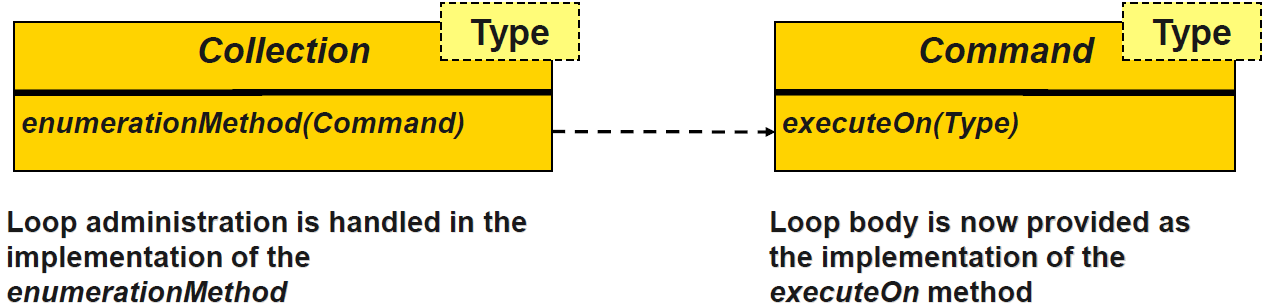
\includegraphics[width=\linewidth]{enumeration_method.png}

\subsubsection{Problem}
\begin{itemize}
    \item Iterationsmanagement wird vom Benutzer der Collection durchgeführt
    \item Vermeidung von Zustandsverwaltung zwischen Collection und Iteration
\end{itemize}

\subsubsection{Intent}
Wie kann eine Sammlung unter Berücksichtigung des Collection state iteriert werden und darüber hinaus die Zustandsverwaltung reduziert werden?

\subsubsection{Solution}
Unterstützt die gekapselte Iteration über eine Sammlung, indem die Verantwortung für die Iteration in einer Methode der Sammlung liegt. Die Methode nimmt ein Command-Objekt, das auf die Elemente der Sammlung angewendet wird \\

\textit{Programming languages already implement Enumeration Method as their loop construct. (e.g. .forEach())}\\

\subsubsection{Consequences}
\textbf{Benefits}
\begin{itemize}
    \item Client ist nicht für Loop-Housekeeping Details verantwortlich
    \item Die Synchronisierung kann auf der Ebene des gesamten Traversals und nicht für jeden einzelnen Elementzugriff vorgenommen werden
\end{itemize}
\vspace{10pt}
\textbf{Liabilities}
\begin{itemize}
    \item Funktionaler Ansatz, komplexere Syntax benötigt
    \item Oft als zu abstrakt für Programmierer betrachtet
    \item Hebelt Command Objects aus
\end{itemize}

\subsection{Batch Method}
\subsubsection{Problem}
\begin{itemize}
    \item Collection und Client (Iteratorbenutzer) befinden sich nicht auf derselben Maschine
    \item Operationsaufrufe sind nicht mehr trivial
\end{itemize}

\subsubsection{Intent}
Wie kann eine Collection über mehrere Ebenen iteriert werden, ohne dass mehr Zeit für die Kommunikation als für die Berechnung benötigt wird?

\subsubsection{Solution}
Gruppiere mehrere Collection-Zugriffe zusammen, um die Kosten für mehrere Einzelzugriffe in einer verteilten Umgebung zu reduzieren. (Z.B. String Builder, oder toString()-Methode, ADO.NET, SQL Cursor)

\begin{itemize}
    \item Define a data structure which groups interface calls on client side
    \item Provide an interface on servant to access groups of elements at once
\end{itemize}
